% !TEX root = /Users/hzd88688126com/Desktop/USFD_Academic-_Report_LaTeX-Template/main.tex
\section{Complex LMS and Widely Linear Modelling}
\subsection{CLMS vs ACLMS}
The Wide Linear Moving Average (WLMA) process with first order is simulated. As shown in Fig.\ref{fig:3_1_a}, the white noise data and filtered data are plotted, which illustrates the circularity of the signal. The white noise is circularity and the filtered signal is not. As to the complex LMS (CLMS) algorithm, only standard strict linear model can be used to estimate the coefficients. Therefore, the learning curve of CLMS is a straight line without convergence. However, augmented CLMS (ACLMS) algorithm applies an additional weight $\mathbf g(n)$, which allows the ACLMS to capture the second-order statistical relationship \cite{mandic}. Thus, the learning curve rapidly decreases and converges at $-300dB$.
\begin{figure}[htp]
    \centering
    \hspace{-0.4cm}
    \begin{subfigure}[b]{0.35\textwidth}
     \centering
     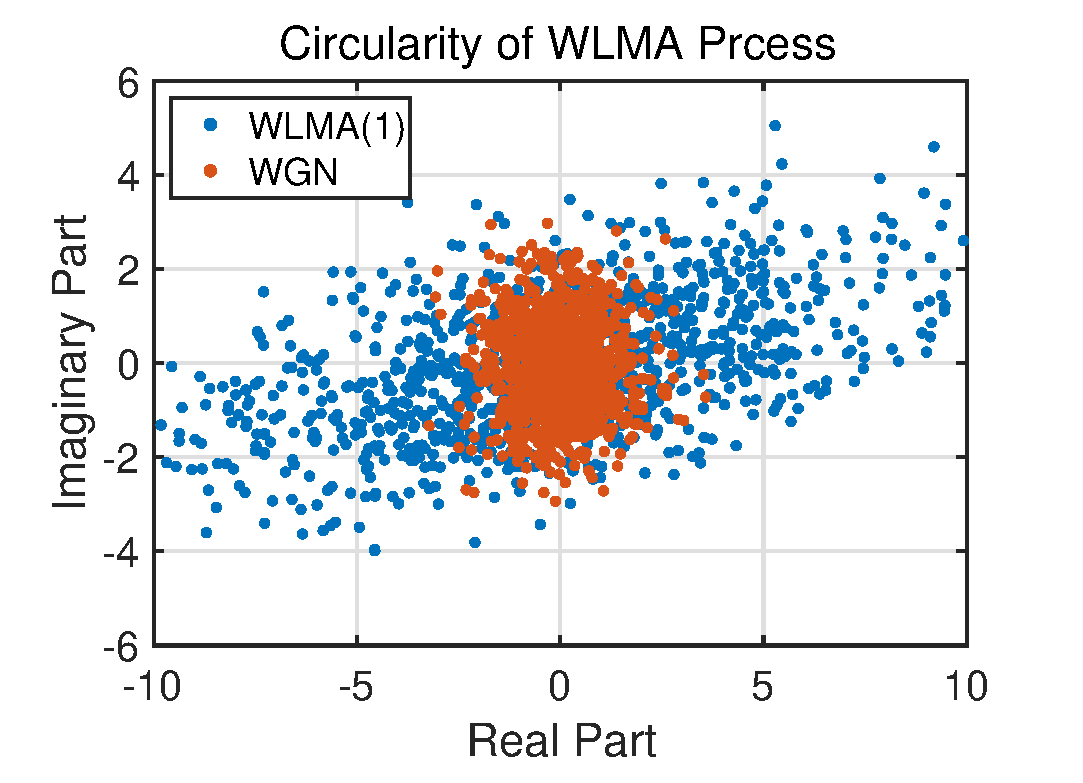
\includegraphics[width=1.2\textwidth]{fig/31/31a1.eps}
    \end{subfigure}
    \hspace{1.4cm}
    \begin{subfigure}[b]{0.35\textwidth}
     \centering
     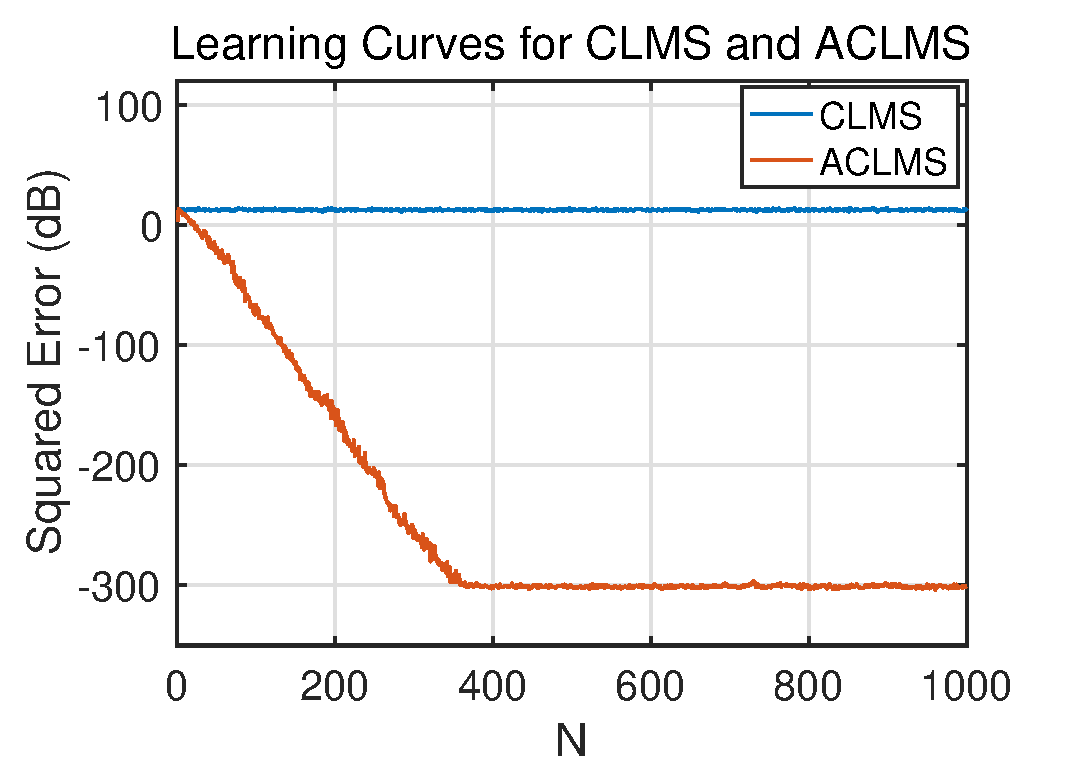
\includegraphics[width=1.2\textwidth]{fig/31/31a2.eps}
    \end{subfigure}  
    \caption{CLMS vs ACLMS: Circularity and learning curves}
    \label{fig:3_1_a}
\end{figure}
\subsection{Wind-speed data}
\begin{figure}[htb]
    \centering
    \hspace{-0.4cm}
    \begin{subfigure}[b]{0.3\textwidth}
     \centering
     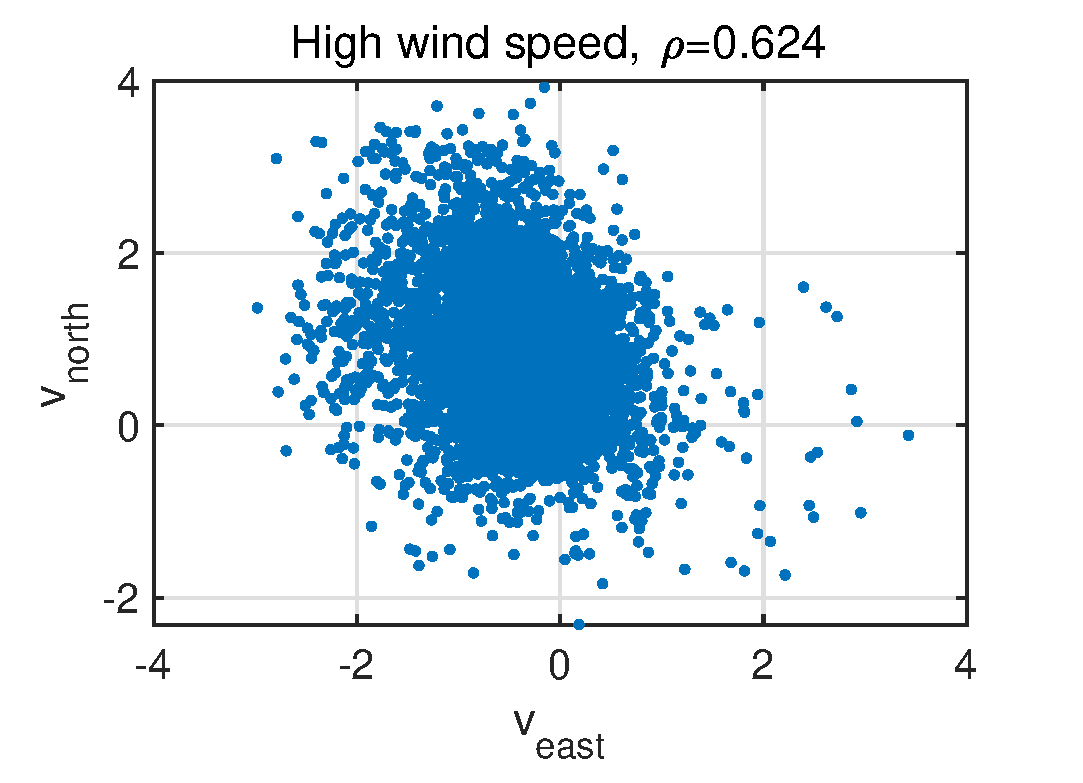
\includegraphics[width=1.2\textwidth]{fig/31/31b1.eps}
    \end{subfigure}
    \hspace{0.4cm}
    \begin{subfigure}[b]{0.3\textwidth}
     \centering
     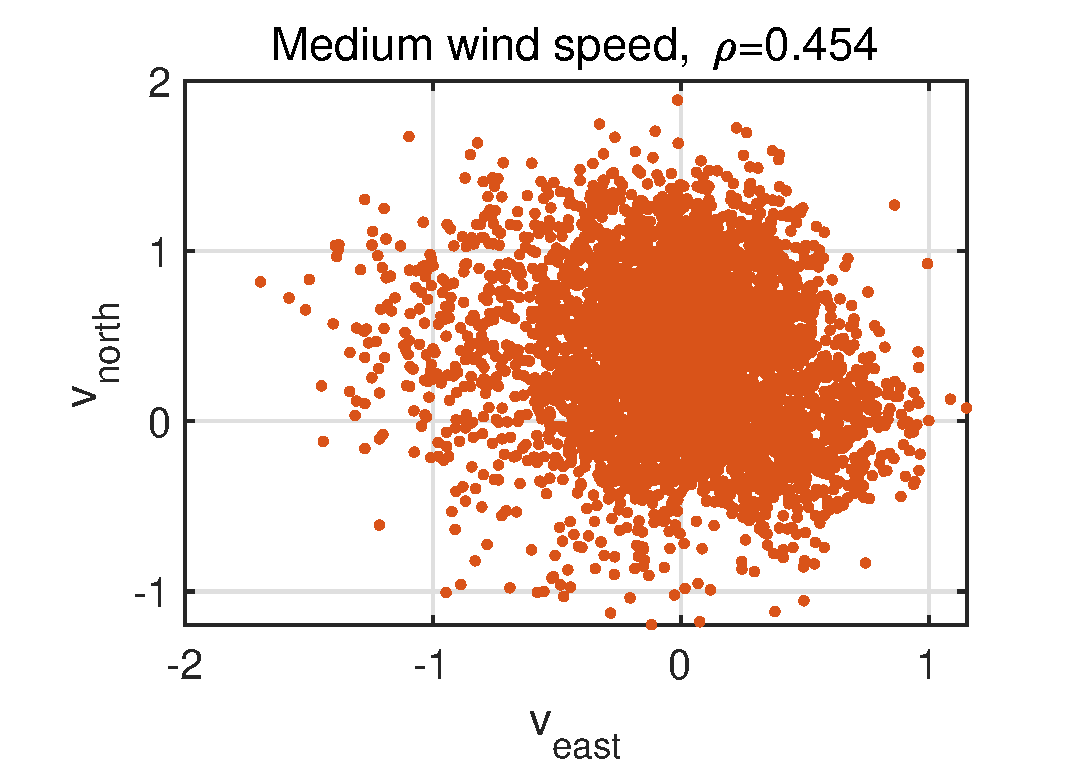
\includegraphics[width=1.2\textwidth]{fig/31/31b2.eps}
    \end{subfigure}  
    \hspace{0.4cm}
    \begin{subfigure}[b]{0.3\textwidth}
     \centering
     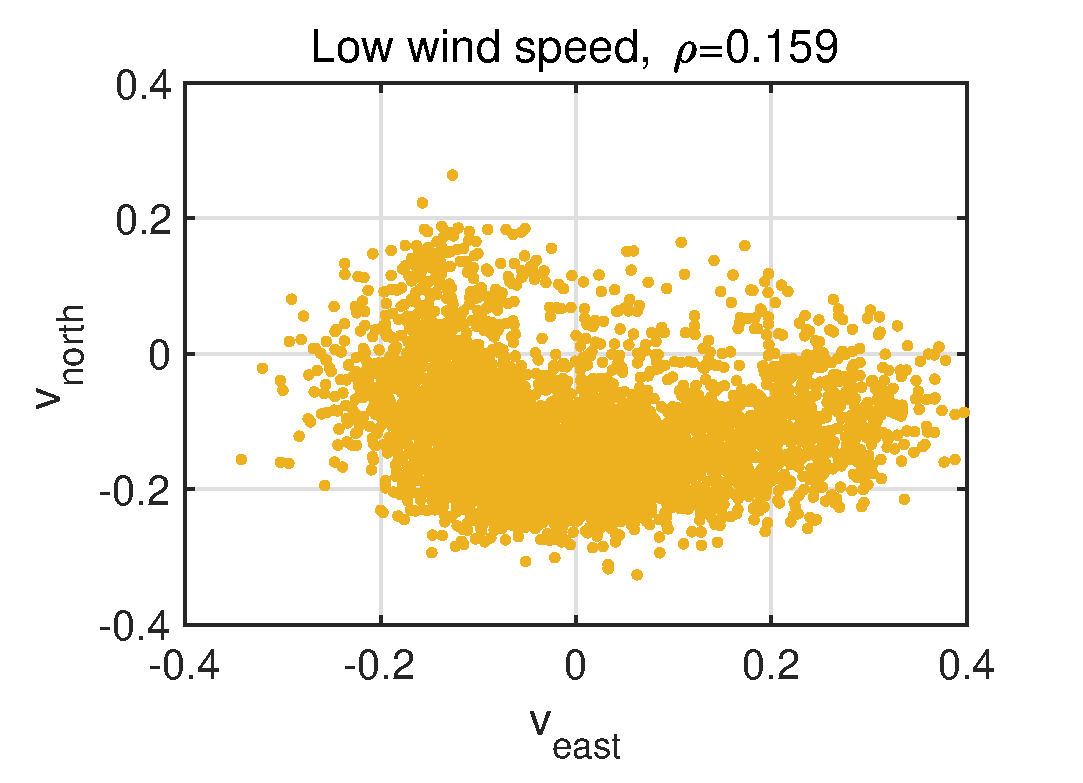
\includegraphics[width=1.2\textwidth]{fig/31/31b3.eps}
    \end{subfigure}  
    \caption{Circularity of Low, Medium and High speed wind data}
    \label{fig:3_1_b1}
\end{figure}
\noindent
The circularity describes the distribution of data. The circular complex random variables will not depend on the angle $\theta$, whose the statistical relationship is remain invariant. As a consequence, the circular model will be easily predicted. Fig.\ref{fig:3_1_b1} plots the scatter data for the three wind regimes with calculated circularity. The high wind regimes has largest circularity coefficient with $\rho=0.624$, while the medium and the low wind data are $\rho=0.454$ and $\rho=0.159$ respectively. The low wind regime has relatively narrow range of distribution, which proved that the model has low degree of non-circularity with the smaller circularity coefficient.
\begin{figure}[htp]
    \centering
    \hspace{-0.4cm}
    \begin{subfigure}[b]{0.3\textwidth}
     \centering
     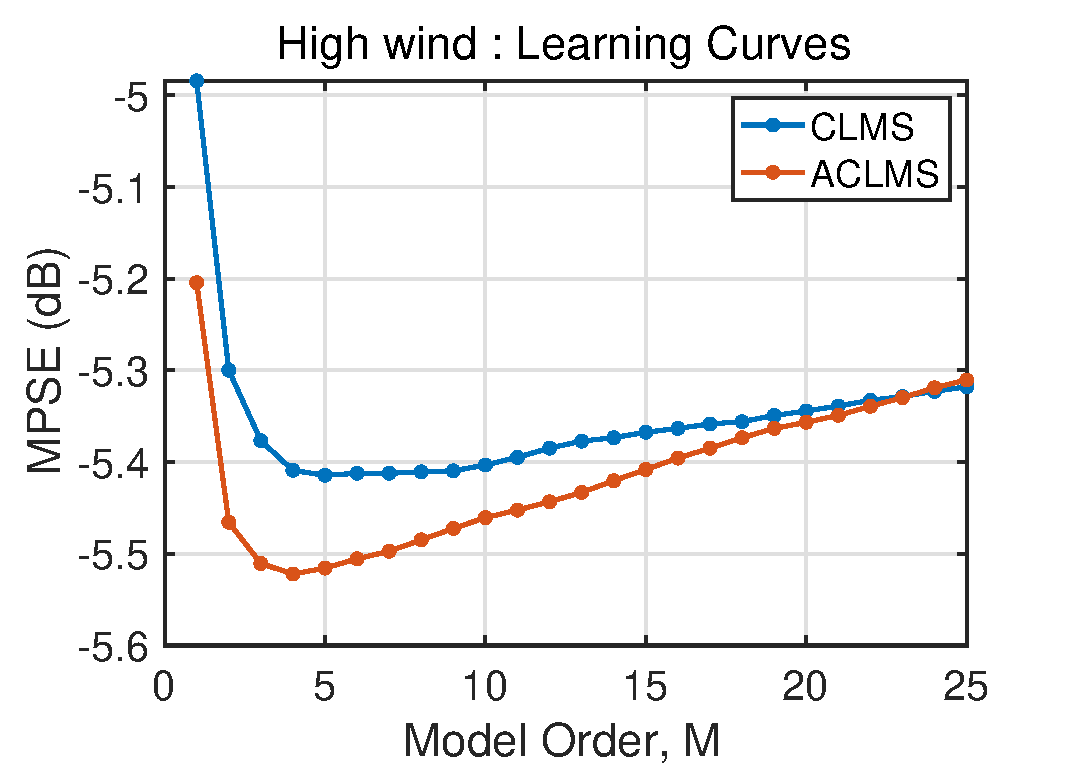
\includegraphics[width=1.2\textwidth]{fig/31/31b4.eps}
    \end{subfigure}
    \hspace{0.4cm}
    \begin{subfigure}[b]{0.3\textwidth}
     \centering
     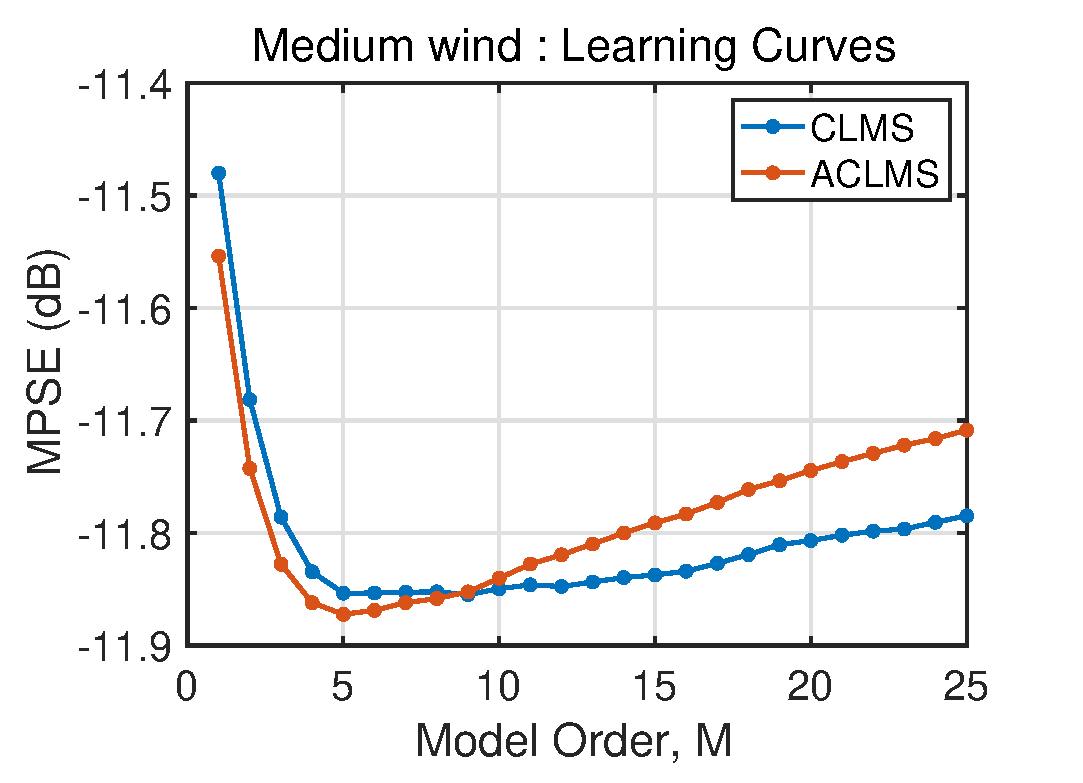
\includegraphics[width=1.2\textwidth]{fig/31/31b5.eps}
    \end{subfigure}  
    \hspace{0.4cm}
    \begin{subfigure}[b]{0.3\textwidth}
     \centering
     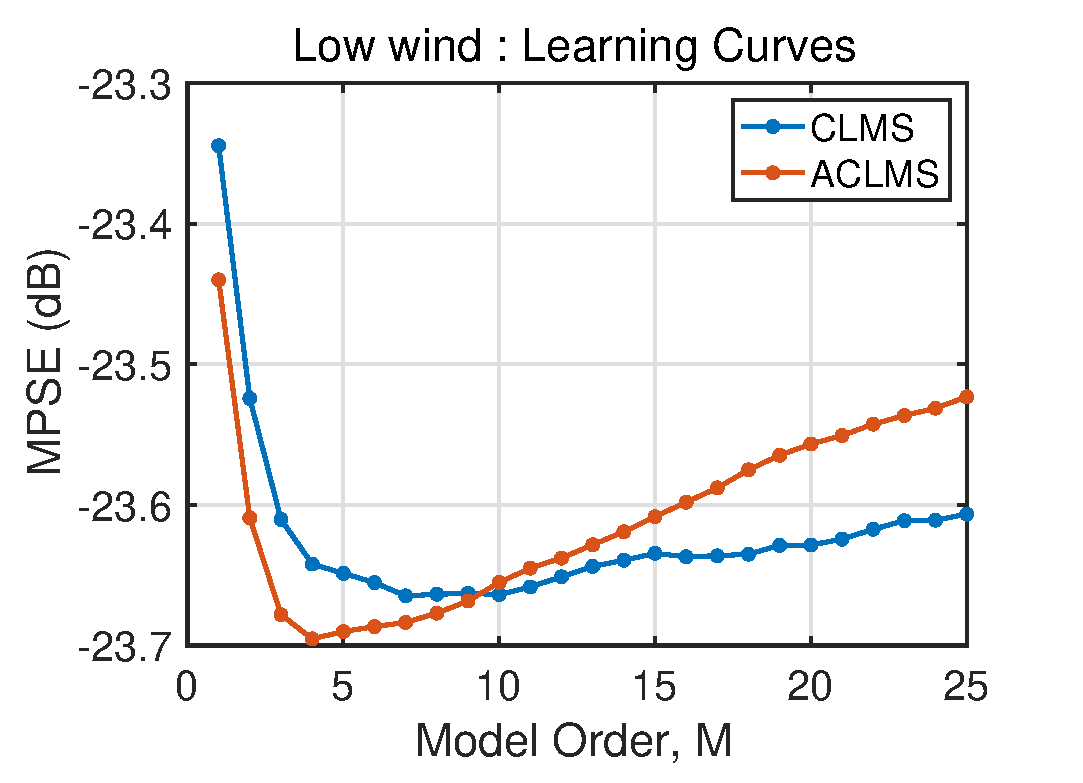
\includegraphics[width=1.2\textwidth]{fig/31/31b6.eps}
    \end{subfigure}  
    \caption{Learning curves of Low, Medium and High speed wind data}
    \label{fig:3_1_b2}
\end{figure}
Applying the CLMS and ACLMS algorithms to the three regimes data, the MSPE curves are illustrated by varying the model order $M\in[1,25]$. It depicts that the wind data with small circularity coefficient has the small squared error. Moreover, the ACLMS algorithm perform has outstanding performance than the CLMS in the beginning range of model order. Afterwards, the minimum errors occur at $M=4,5$ and the model is getting to suffer over-fitting issues, resulting in growing error. In addition, the ACLMS has extra degrees of freedom, which leads to the advanced over-fitting than the CLMS. Therefore, the optimal model order for the wind regimes data are $M\in[3,6]$.
\subsection{Balanced and Unbalanced System}
\begin{figure}[htb]
    \centering
    \hspace{-0.4cm}
    \begin{subfigure}[b]{0.3\textwidth}
     \centering
     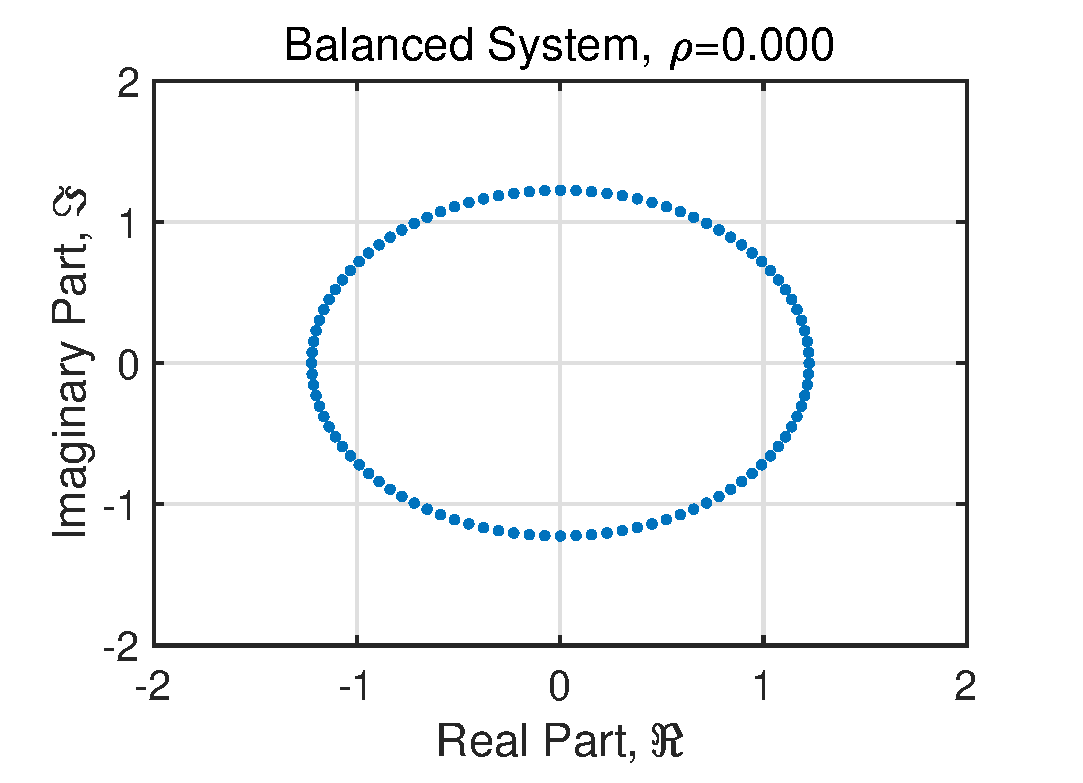
\includegraphics[width=1.2\textwidth]{fig/31/31c1.eps}
    \end{subfigure}
    \hspace{1.4cm}
    \begin{subfigure}[b]{0.3\textwidth}
     \centering
     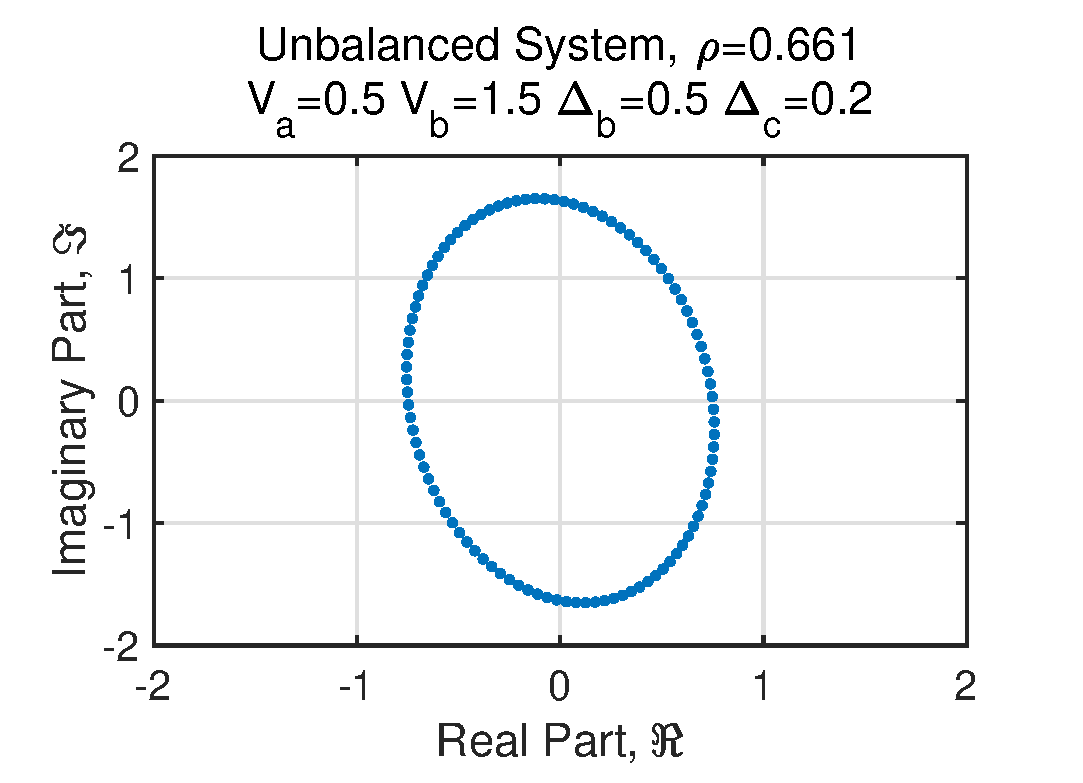
\includegraphics[width=1.2\textwidth]{fig/31/31c2.eps}
    \end{subfigure}  
    \caption{Examples of Balanced and Unbalanced System}
    \label{fig:3_1_c1}
\end{figure}
\begin{figure}[htb]
    \centering
    \hspace{-0.4cm}
    \begin{subfigure}[b]{0.3\textwidth}
     \centering
     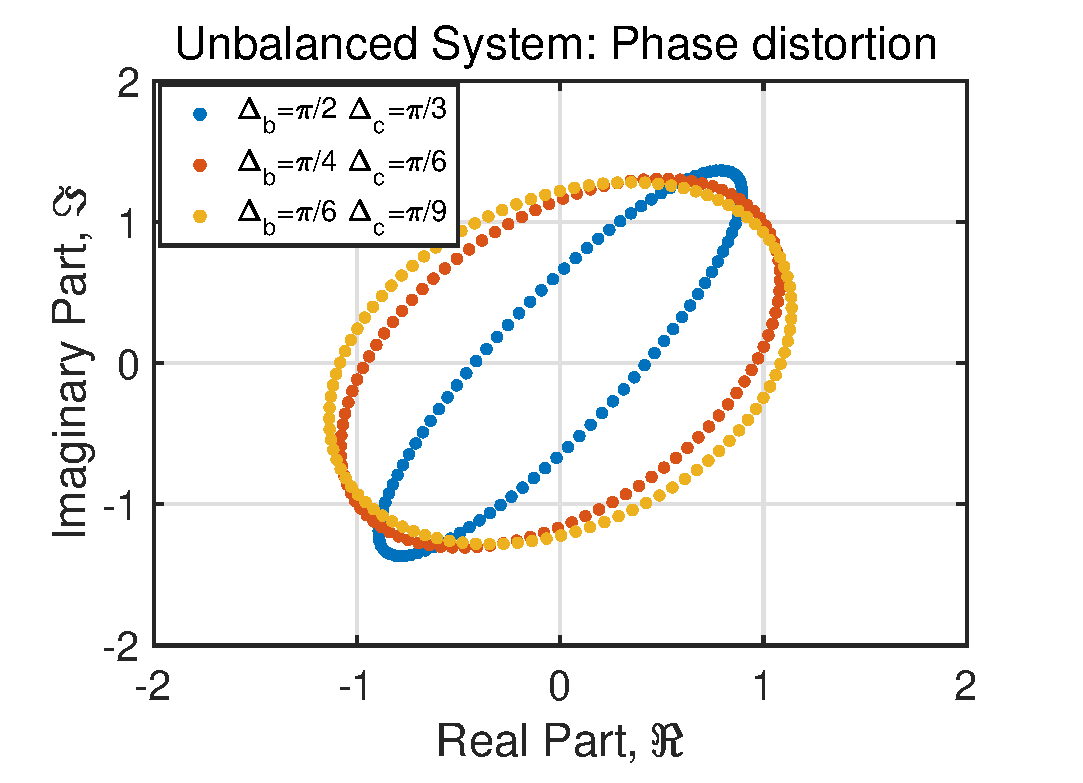
\includegraphics[width=1.2\textwidth]{fig/31/31c3.eps}
    \end{subfigure}
    \hspace{1.4cm}
    \begin{subfigure}[b]{0.3\textwidth}
     \centering
     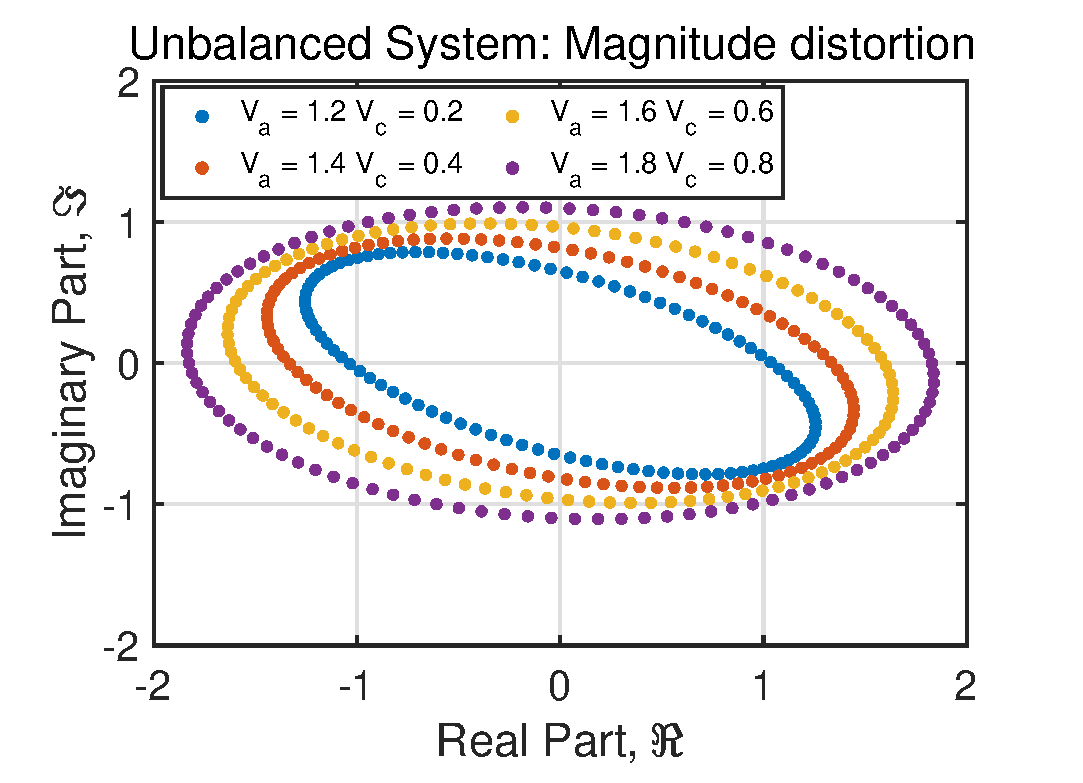
\includegraphics[width=1.2\textwidth]{fig/31/31c4.eps}
    \end{subfigure}   
    \caption{Unbalanced system with phase and magnitude distortion}
    \label{fig:3_1_c2}
\end{figure}
\noindent
According to the Clarke Transformation, the circularity example diagrams of balanced and unbalanced system are plotted as illustrated in Fig.\ref{fig:3_1_c1}. The amplitude of three phase voltages are seleceted as $V_a=0.5$, $V_b=1.5$, $V_c=1$ and the phase distortions are $\Delta_b=0.5$ and $\Delta_c=0.2$. Totally 2000 samples with sample frequency $f_s=5000Hz$ are simulated. For the balanced system, the magnitude of phase voltage are equal ($V_a=V_b=V_c$), meanwhile there is no phase distortion with $\Delta_b=\Delta_c=0$. Therefore, changing the voltage magnitude and phase distortion causes a large circularity coefficient $\rho=0.661$ shown in Fig.\ref{fig:3_1_c1}(b). Fig.\ref{fig:3_1_c2} depicts the effect of magnitude and phase distortion on circularity.
\subsection{Derivation of nominal frequency}
According to the zero-sequence voltage $v_0$ under balanced conditions given by
\begin{align}
v(n)=\sqrt{\frac{3}{2}}Ve^{j(2\pi\frac{f_o}{f_s}n+\phi)}\label{eq:vol}
\end{align}
Thus, the strict Linear model can be derived as
\begin{align}
v(n+1)&=h^*(n)v(n)\notag\\
\sqrt{\frac{3}{2}}Ve^{j(2\pi\frac{f_o}{f_s}(n+1)+\phi)}&=h^*(n)\sqrt{\frac{3}{2}}Ve^{j(2\pi\frac{f_o}{f_s}n+\phi)}\notag\\
\end{align}
Simplify both sides based on exponents rules, 
\begin{align}
e^{j2\pi\frac{f_o}{f_s}}&=h^*(n)\notag\\
e^{j2\pi\frac{f_o}{f_s}}&=|h^*(n)|e^{j\angle{\theta(h^*(n))}}
\label{eq:balan}
\end{align}
Observing Eq.\ref{eq:balan}, the equation will only satisfy if and only if that the magnitude and the angle are equal on both sides. Due to the angle of complex number $h^*(n)$ defined as $\angle \theta(h^*(n)) =\tan^{-1}(\frac{\Im\{h^*(n)\}}{\Re\{h^*(n)\}})$, the equation below can be derived from Eq.\ref{eq:balan}.
\begin{align}
2\pi\frac{f_o}{f_s}&=\tan^{-1}(\frac{\Im\{h^*(n)\}}{\Re\{h^*(n)\}})\notag\\
f_o(n)&=-\frac{f_s}{2\pi}\tan^{-1}(\frac{\Im\{h^(n)\}}{\Re\{h(n)\}})
\label{eq:fb}
\end{align}
However, the negative sign in the EQ.\ref{eq:fb} is use{}d to guarantee the estimated nominal frequency $f_o$ to be positive, since the imaginary part of weight $h(n)$ may be negative.
As to the unbalanced system, the Clarke Transform is used instead of Eq.\ref{eq:vol}
\begin{align}
v(n)=A(n)e^{j(2\pi\frac{f_o}{f_s}n+\phi)}+B(n)e^{-j(2\pi\frac{f_o}{f_s}n+\phi)}\label{eq:unvol}
\end{align}
Hence, the widely linear model $v(n+1)=h^*(n)v(n)+g^*(n)v^*(n)
$ can be expressed as
\begin{align}
&A(n+1)e^{j(2\pi\frac{f_o}{f_s}(n+1)+\phi)}+B(n+1)e^{-j(2\pi\frac{f_o}{f_s}(n+1)+\phi)}\notag\\
=&h^*(n)\left\{A(n)e^{j(2\pi\frac{f_o}{f_s}n+\phi)}+B(n)e^{-j(2\pi\frac{f_o}{f_s}n+\phi)}\right\}+g^*(n)\left\{A^*(n)e^{-j(2\pi\frac{f_o}{f_s}n+\phi)}+B^*(n)e^{j(2\pi\frac{f_o}{f_s}n+\phi)}\right\}
\end{align}
Afterwards, the terms with identical exponent term are same, which are
\begin{align}
A(n+1)e^{j(2\pi\frac{f_o}{f_s}(n+1)+\phi)}&=[h^*(n)A(n)+g^*(n)B^*(n)]e^{j(2\pi\frac{f_o}{f_s}n+\phi)}\label{eq:a1}\\
B(n+1)e^{-j(2\pi\frac{f_o}{f_s}(n+1)+\phi)}&=[h^*(n)B(n)+g^*(n)A^*(n)]e^{-j(2\pi\frac{f_o}{f_s}n+\phi)}\label{eq:b1}
\end{align}
For a time sequence unbalanced system, the term $A(n+1)$ and $B(n+1)$ can be assumed that $A(n+1)\approx A(n)$ and $B(n+1)\approx B(n)$ respectively. Thus, the Eq.\ref{eq:a1} and \ref{eq:b1} can be simplified as
\begin{align}
e^{j2\pi\frac{f_o}{f_s}}&=\frac{h^*(n)A(n)+g^*(n)B^*(n)}{A(n+1)} \approx h^*(n)+g^*(n)\frac{B^*(n)}{A(n)}\label{eq:a}\\
e^{-j2\pi\frac{f_o}{f_s}}&=\frac{h^*(n)B(n)+g^*(n)A^*(n)}{B(n+1)} \approx h^*(n)+g^*(n)\frac{A^*(n)}{B(n)}\label{eq:b}
\end{align}
In addition, the Eq.\ref{eq:b} is the conjugate term of Eq.\ref{eq:a}. Thus, 
\begin{align}
\left\{h^*(n)+g^*(n)\frac{B^*(n)}{A(n)}\right\}^* & =h^*(n)+g^*(n)\frac{A^*(n)}{B(n)}\notag\\
h(n)+g(n)\frac{B(n)}{A^*(n)}&=h^*(n)+g^*(n)\frac{A^*(n)}{B(n)}\label{eq:b2}
\end{align}
Let the term $\frac{B(n)}{A^*(n)}=X$ for simplicity. Multiply $\frac{B(n)}{A^*(n)}$ on both sides, a quadratic equation of X is formed.
\begin{align}
h(n)\frac{B(n)}{A^*(n)}+g(n)\left |\frac{B(n)}{A^*(n)}\right|^2&=h^*(n)\frac{B(n)}{A^*(n)}+g^*(n)\notag\\
g(n)X^2+[h(n)-h^*(n)]X&+g^*(n)=0\notag\\
g(n)X^2+2\Im \{h(n)\}X&+g^*(n)=0
\end{align}
Therefore, the solution of term $X$ is
\begin{align}
\frac{B(n)}{A^*(n)}=X
&=\frac{-2\Im\{h(n)\}\pm j\sqrt{4\Im^2\{h(n)\}-4g^*(n)g(n)}}{2g(n)}\notag\\
&=\frac{-\Im\{h(n)\}\pm j\sqrt{\Im^2\{h(n)\}-|g(n)|^2}}{g(n)}\label{eq:X}
\end{align}
Substituting the solution into Eq.\ref{eq:b2} and \ref{eq:b} and keeping the corresponding sign, the equation below can be obtained.
\begin{align}
e^{-j2\pi\frac{f_o}{f_s}}
&\approx h^*(n)+g^*(n)\frac{A^*(n)}{B(n)}\notag\\
&=h(n)+g(n)\frac{B(n)}{A^*(n)}\notag\\
&=h(n)+g(n)\frac{-\Im\{h(n)\}- j\sqrt{\Im^2\{h(n)\}-|g(n)|^2}}{g(n)}\notag\\
&=\Re\{h(n)\}- j\sqrt{\Im^2\{h(n)\}-|g(n)|^2}\label{eq:final}
\end{align}
Thus, transform the complex number into exponential expression.
\begin{align}
-2\pi\frac{f_o}{f_s}&=-\tan^{-1}\left\{ \frac{\sqrt{\Im^2\{h(n)\}-|g(n)|^2}}{\Re\{h(n)\}}\right\} \notag\\
f_o(n)&=\frac{f_s}{2\pi}\tan^{-1}\left\{ \frac{\sqrt{\Im^2\{h(n)\}-|g(n)|^2}}{\Re\{h(n)\}}\right\}
\end{align}
\subsection{ACLMS and CLMS on frequency estimation}
As proofed on previous question, the nominal frequency can be estimated based on the ACLMS and CLMS algorithms. The theoretical nominal frequency is set to $50Hz$. Fig.\ref{fig:3_1_e1} illustrated the squared errors and estimation curves after applying these two algorithms. Both of algorithms can correctly estimate the $50Hz$ at stead-state without bias. The learning curve for the CLMS converges faster than the applying the ACLMS algorithm. Since there is an additional weight $\mathbf g(n)$ of the ACLMS needed to be considered, the frequency estimation has large bias at the beginning time index. 
\begin{figure}[htb]
    \centering
    \hspace{-0.4cm}
    \begin{subfigure}[b]{0.32\textwidth}
     \centering
     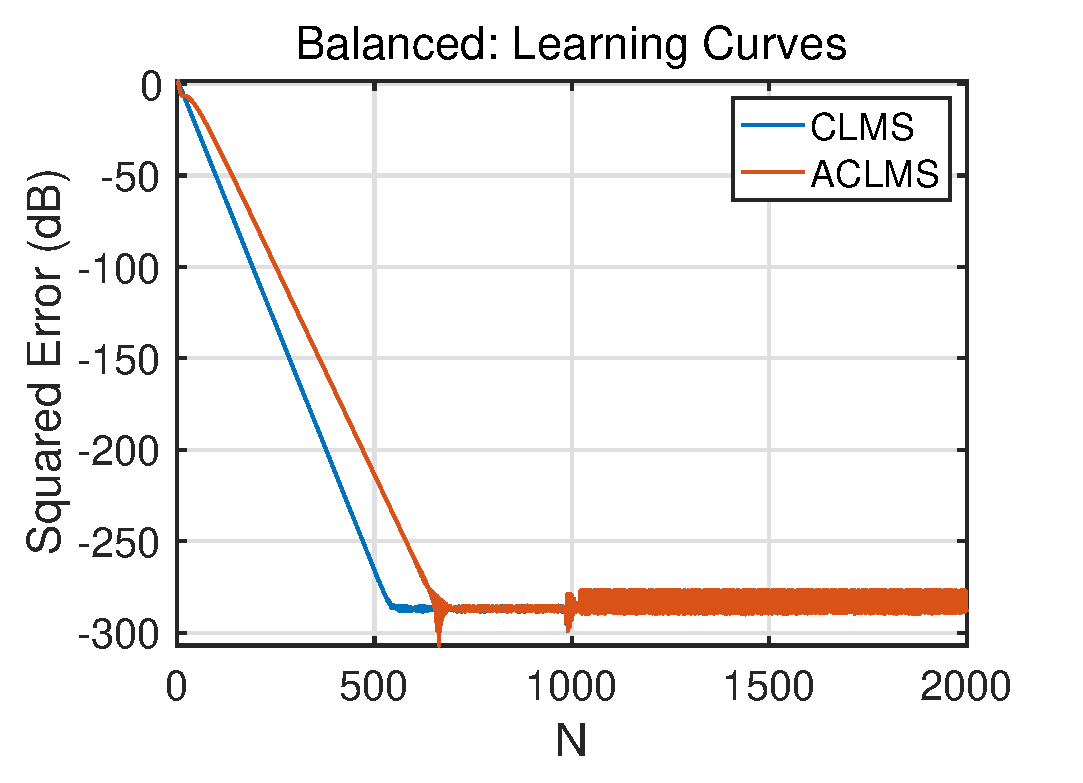
\includegraphics[width=1.2\textwidth]{fig/31/31e1.eps}
    \end{subfigure}
    \hspace{1.4cm}
    \begin{subfigure}[b]{0.32\textwidth}
     \centering
     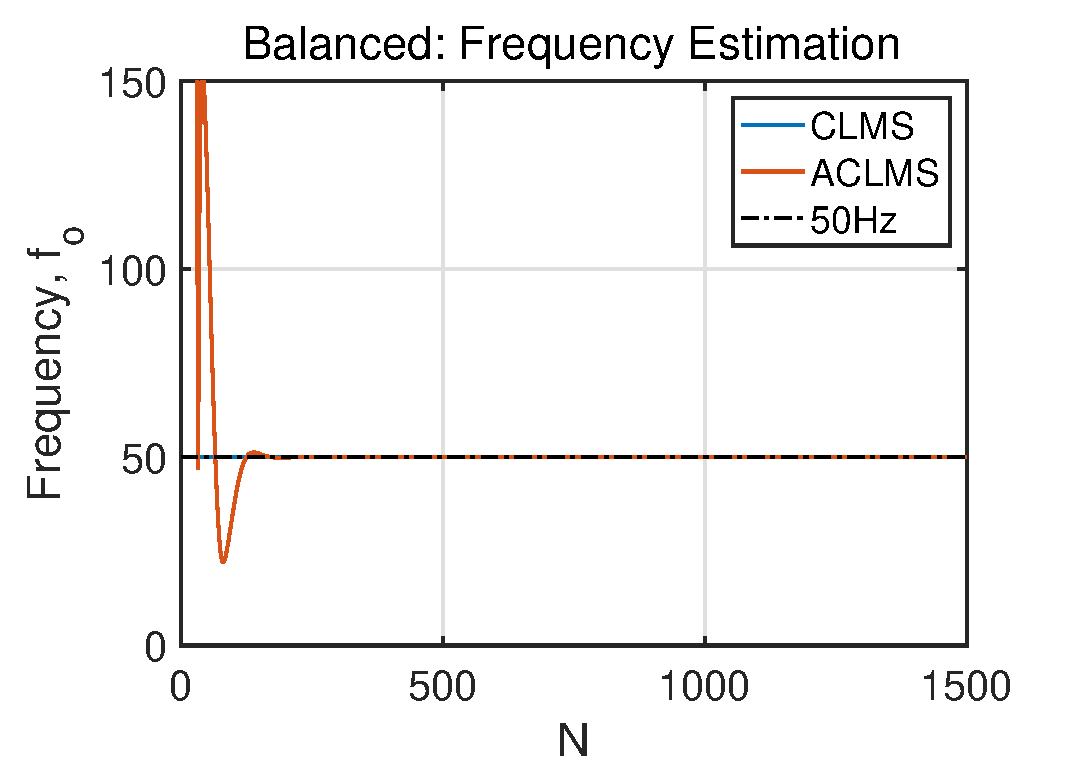
\includegraphics[width=1.2\textwidth]{fig/31/31e2.eps}
    \end{subfigure}  
    \caption{ACLMS vs CLMS: Learning curves and estimated frequency for balanced system}
    \label{fig:3_1_e1}
\end{figure}\\
When dealing with the unbalanced system as shown in Fig.\ref{fig:3_1_c1}(b), the CLMS algorithm can not capture the non-circularity data, resulting in non-update for learning. Thus, the frequency estimation has a bias and oscillation below $50Hz$. However, the convergence speed of the CLMS is much fast than the ACLMS. As to the ACLMS algorithm, the learning curve converges after 1800 samples with large ripples, which is caused by the distortion of the system. As to the frequency estimation, large oscillations occur in the beginning of 400 samples. Afterwards, the ACLMS converges to the true nominal frequency without bias and overshooting. In general, the ACLMS algorithm has sufficient performance that can replace the CLMS when dealing with both circularity and non-circularity data.
\begin{figure}[htb]
    \centering
    \hspace{-0.4cm}
    \begin{subfigure}[b]{0.32\textwidth}
     \centering
     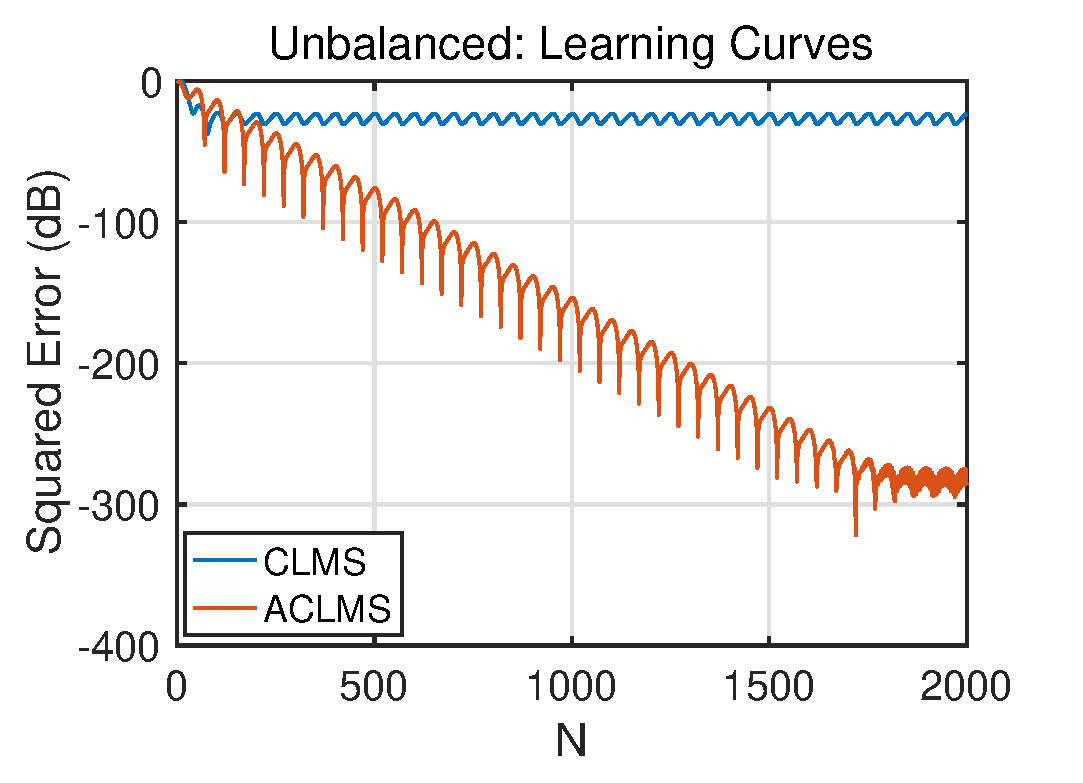
\includegraphics[width=1.2\textwidth]{fig/31/31e3.eps}
    \end{subfigure}
    \hspace{1.4cm}
    \begin{subfigure}[b]{0.32\textwidth}
     \centering
     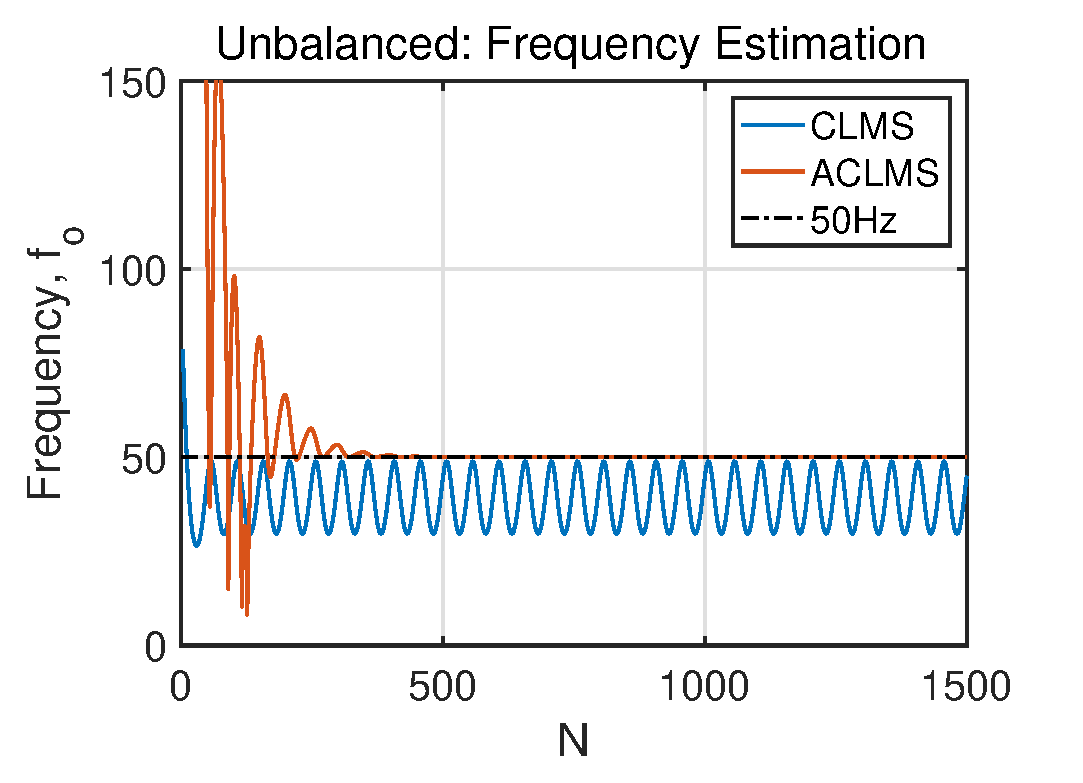
\includegraphics[width=1.2\textwidth]{fig/31/31e4.eps}
    \end{subfigure}  
    \caption{ACLMS vs CLMS: Learning curves and estimated frequency for unbalanced system}
    \label{fig:3_1_e2}
\end{figure}









